\section{Conclusion}
%\textit{Includes intelligent evaluation of your system’s performance (success \& failure cases shown), and next steps to take, given more time, both in the short- (2-3 wks) and long-term (up to a year).}

Our system successfully interpreted the equations seen in the following images.

\begin{minipage}[h!]{.9\linewidth}%
\begin{minipage}[h!]{0.49\textwidth}%
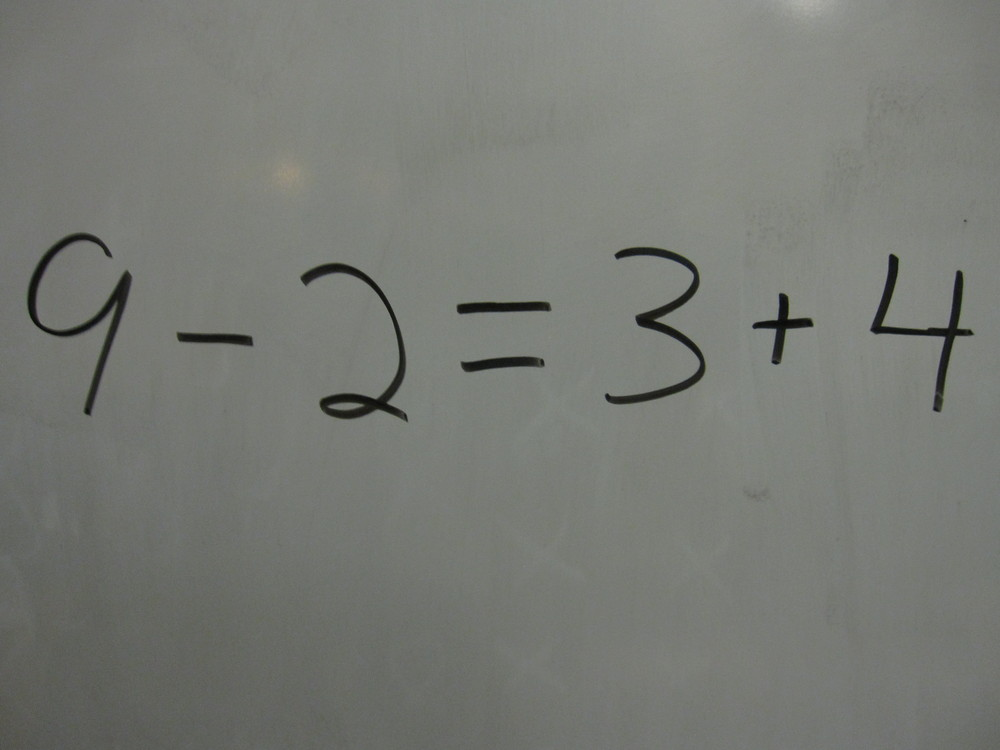
\includegraphics[width=\textwidth]{images/img_001.jpg}
\end{minipage}
\begin{minipage}[h!]{0.49\textwidth}%
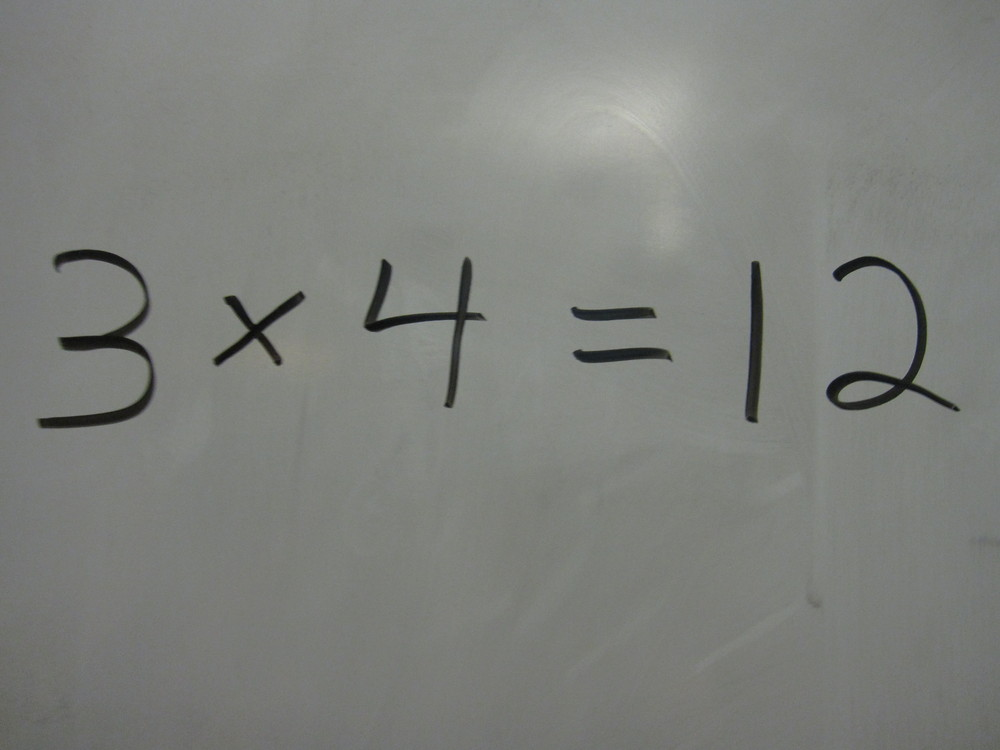
\includegraphics[width=\linewidth]{images/img_002.jpg}
\end{minipage}
\vfill
\begin{minipage}[h!]{0.49\textwidth}%
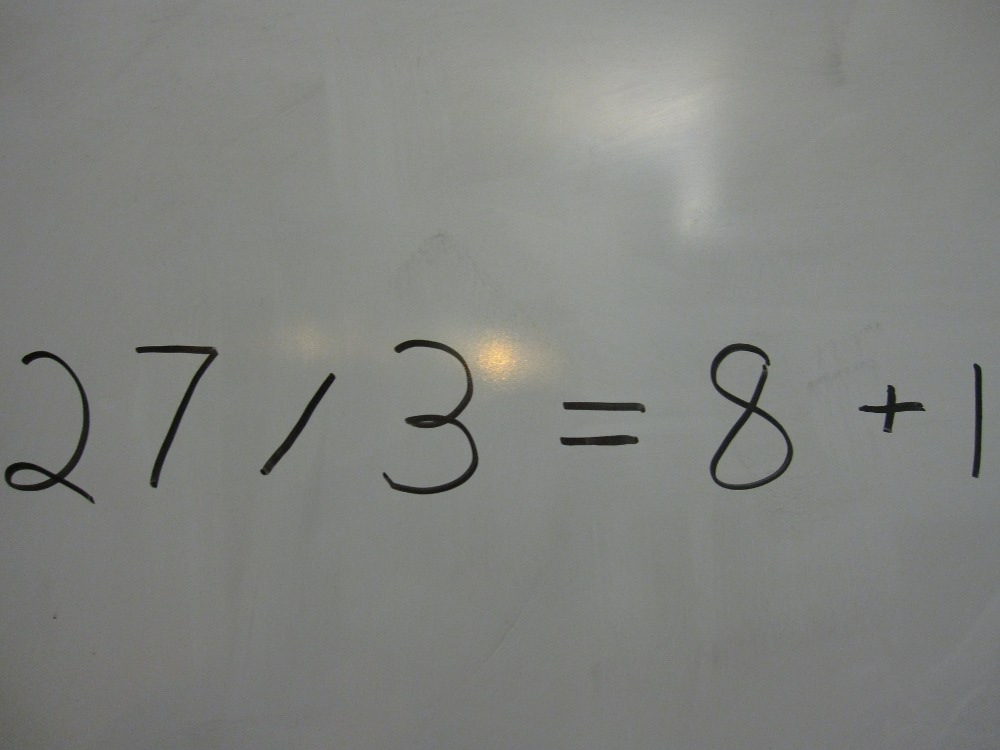
\includegraphics[width=\textwidth]{images/img_003.jpg}
\end{minipage}
\begin{minipage}[h!]{0.49\textwidth}%
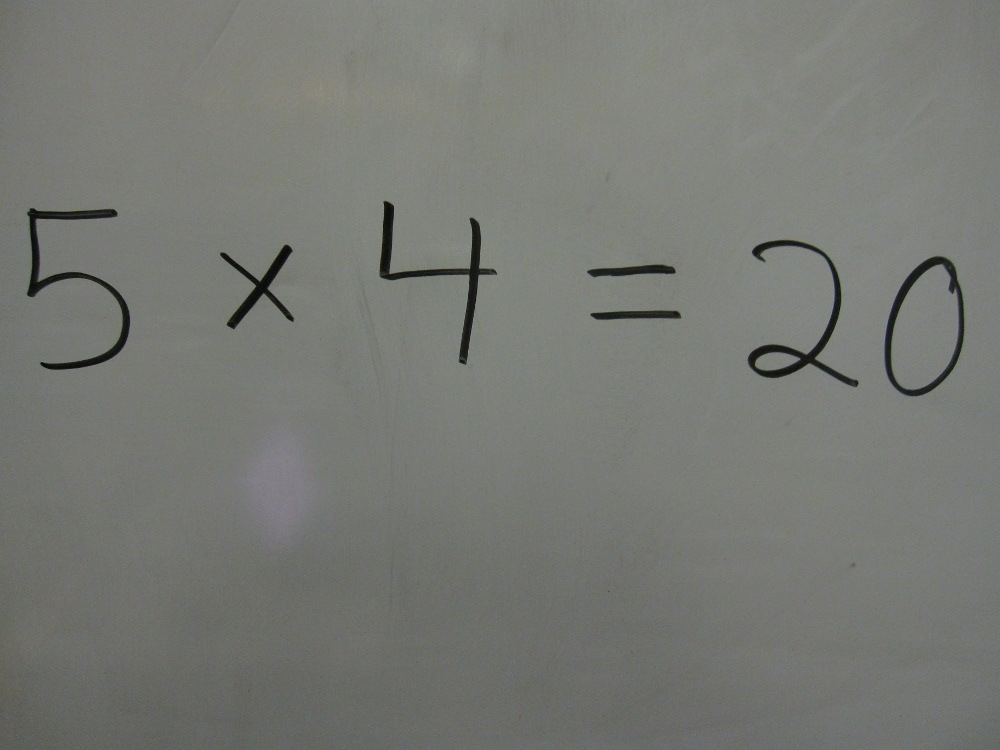
\includegraphics[width=\linewidth]{images/img_004.jpg}
\end{minipage}
\captionof{figure}{Successfully interpreted images}
\vspace{5 mm}
\end{minipage}

Clearly these images are not overly contrived. They represent a variety of variably sized symbols located at different locations in the image. We had excellent success when we consistently used these large block symbols.

\addImage{images/broken.jpg}{Unsuccessfully classified image. Result: (5+7=9*4)}{miss}{.21}

However, our system certainly has restrictions on its robustness. For instance, the image seen in Fig. \ref{miss} was misclassified because the 29 was grouped together as one symbol. This essentially made the resulting classification nonsense.  

As seen increasing the robustness of image segmentation is certainly a portion of the project that needs improvement. Given two to three weeks more to work on a project this would certainly be an area of focus. We would need to devise some systematic approach that would also allow for the easy addition of new symbols. Our ultimate long term goal would be to provide support for a very large set of mathematical symbols and create an intuitive method for each user to train the classifier with their own handwriting.